% ============================================================================
% JURNAL TUGAS AKHIR - D3RPLA
% Template LaTeX gaya IEEE untuk artikel jurnal Tugas Akhir jalur Publikasi
% Program Studi D3 Rekayasa Perangkat Lunak Aplikasi
% Fakultas Ilmu Terapan, Universitas Telkom
%
% Sumber: Template Jurnal_7.docx (milik Prodi D3RPLA, tidak ikut dipush ke repo).
% ============================================================================

\documentclass[conference,a4paper,10pt]{IEEEtran}

% --- Engine & jenis huruf: Times New Roman (mengikuti DOCX referensi) ---
% XeLaTeX/LuaLaTeX memakai Times New Roman sistem bila tersedia; pdfLaTeX
% memakai TeX Gyre Termes (clone Times New Roman, metrik kompatibel).
\usepackage{iftex}
\ifPDFTeX
  \usepackage{tgtermes}
\else
  \usepackage{fontspec}
  \IfFontExistsTF{Times New Roman}{\setmainfont{Times New Roman}}{%
    \IfFontExistsTF{TeX Gyre Termes}{\setmainfont{TeX Gyre Termes}}{}}
\fi

% --- Paket standar ---
\usepackage{cite}
\usepackage{amsmath,amssymb,amsfonts}
\usepackage{algorithmic}
\usepackage{graphicx}
\usepackage{textcomp}
\usepackage{xcolor}
\usepackage{hyperref}
\usepackage{url}
\usepackage{array}
\usepackage{booktabs}
\usepackage{tabularx}
\usepackage{float}

\graphicspath{{assets/jurnal/}{assets/}}

\hypersetup{colorlinks=true,linkcolor=black,urlcolor=blue,citecolor=black}

\begin{document}

% ===================== JUDUL & PENULIS =====================
\title{JUDUL TUGAS AKHIR}

\author{
    \IEEEauthorblockN{1\textsuperscript{st} Nama Mahasiswa}
    \IEEEauthorblockA{School of Applied Science\\
    Telkom University\\
    Bandung, Indonesia\\
    email@student.telkomuniversity.ac.id}
    \and
    \IEEEauthorblockN{2\textsuperscript{nd} Nama Pembimbing 1}
    \IEEEauthorblockA{School of Applied Science\\
    Telkom University\\
    Bandung, Indonesia\\
    email@telkomuniversity.ac.id}
    \and
    \IEEEauthorblockN{3\textsuperscript{rd} Nama Pembimbing 2}
    \IEEEauthorblockA{School of Applied Science\\
    Telkom University\\
    Bandung, Indonesia\\
    email@telkomuniversity.ac.id}
}

\maketitle

% ===================== ABSTRACT =====================
\begin{abstract}
Lorem ipsum dolor sit amet, consectetur adipiscing elit. Cras ultricies viverra
lectus, nec porttitor dolor. Nullam fermentum ullamcorper arcu, ac condimentum
nisi dignissim vel. Pellentesque elementum fermentum diam, in sodales lorem
tristique non. Ut iaculis tellus elit, in suscipit mauris ultrices id. Nam ac
eros urna. Maecenas fermentum ligula quis justo dictum, quis pulvinar. Sed
commodo malesuada sapien, sit amet porttitor lectus aliquet a. Suspendisse
faucibus magna augue, at sodales ex commodo ut. Etiam purus ipsum, mollis sit
amet metus in, iaculis euismod odio. Fusce mollis sit amet metus sit amet
sagittis. Aliquam id tempor erat. Aenean ac sem sed mi mollis faucibus. Sed
mollis turpis dolor. Mauris sit amet eros et sem luctus hendrerit. Phasellus
sollicitudin urna dolor, vitae tincidunt purus condimentum et. Integer dictum
eros sed ligula rhoncus cursus sit amet quis nibh. Cras tincidunt venenatis
risus et viverra. Suspendisse purus magna, fermentum a leo et, vestibulum
tempor velit. Mauris porta dolor eros, sed sodales sapien auctor at. Vestibulum
eu blandit neque.
\end{abstract}

\begin{IEEEkeywords}
    keyword1, keyword2, keyword3, keyword4
\end{IEEEkeywords}

% ===================== PENDAHULUAN =====================
\section{Pendahuluan}
Berdasarkan data yang dihimpun oleh Kementerian Kesehatan, penyandang
disabilitas di Indonesia kurang lebih berjumlah 6 juta jiwa, dimana di dalamnya
terdapat sekitar 472 ribu jiwa penyandang tunarungu~\cite{ref1}. Tunarungu adalah
suatu kondisi dimana seseorang mengalami kekurangan indra pendengaran sehingga
tidak mampu menangkap bunyi. Sebagai akibat terhambatnya perkembangan pendengaran,
seorang tunarungu biasanya juga terhambat kemampuan bicara dan bahasanya,
sehingga seorang tunarungu akan lambat dan sulit dalam hal berkomunikasi~\cite{ref2}.

Di Indonesia, bahasa isyarat yang digunakan oleh kalangan tunarungu untuk
komunikasi terdapat 2 jenis yaitu Bahasa Isyarat Indonesia (BISINDO) dan Sistem
Isyarat Bahasa Indonesia (SIBI). SIBI merupakan bahasa yang biasa dipakai di
Sekolah Luar Biasa (SLB) karena SIBI merupakan bahasa isyarat yang resmi
berdasarkan aturan bahasa isyarat di Indonesia. Terdapat sebanyak 2.070 SLB di
Indonesia dengan jumlah siswa penyandang tunarungu sebanyak 24.374 siswa, yang
merupakan siswa penyandang disabilitas terbanyak ke-2 di Indonesia setelah
tunagrahita~\cite{ref3}.

Namun sayangnya, pembelajaran kosakata baru SIBI pada SLB masih menggunakan
cara konvensional yaitu masih menggunakan kamus bahasa isyarat, dimana kamus
tersebut harganya mencapai 2,5 juta rupiah~\cite{ref4} dan sulit dimengerti
karena hanya menggunakan gambar dengan panduan gerakan berupa teks keterangan.
Apalagi di masa pandemi, pembelajaran harus dilakukan secara daring, sehingga
mengganggu proses pembelajaran karena siswa sangat bergantung pada visual dalam
belajar. Apabila koneksi internet siswa sedang tidak stabil, akan mengganggu
proses pembelajaran.

Oleh karena itu dibuatlah aplikasi yang bernama SIBIKU, yaitu sebuah aplikasi
Android yang merupakan Kamus Sistem Isyarat Bahasa Indonesia (SIBI) dengan
gambar bergerak dan dilengkapi dengan morse getaran. Aplikasi ini dibuat dengan
tujuan agar dapat membantu anak-anak penyandang tunarungu untuk belajar
kosakata bahasa isyarat. Pada aplikasi SIBIKU terdapat beberapa fitur yang
berbeda dengan aplikasi-aplikasi yang sudah ada, namun utamanya yaitu fitur kata
menggunakan gambar bergerak yang bisa ditambah kapan saja oleh guru/admin dari
aplikasi SIBIKU Admin.

% ===================== PENELITIAN TERKAIT =====================
\section{Penelitian Terkait}
Lorem ipsum dolor sit amet, consectetur adipiscing elit. Fusce sit amet magna
in diam finibus convallis. Nulla velit erat, efficitur vitae maximus ut,
imperdiet nec dolor. Sed dui ligula, rutrum eget quam eu, elementum finibus
ipsum. Integer sed porta risus, sit amet tristique neque. Nunc vel convallis
eros. Aliquam luctus lorem eu nisl porta dignissim sit amet ac tortor. Cras
auctor nibh ac aliquet interdum. Donec cursus mauris risus. Morbi laoreet augue
ac massa feugiat, ut laoreet magna semper. Ut non suscipit ante, et luctus
risus. Mauris porta tempus dictum.

Vivamus tincidunt id nibh non euismod. Proin lectus orci, tempus ac rhoncus
vitae, luctus vel dolor. Phasellus faucibus porta urna, posuere consequat eros
dapibus at. Ut felis nisl, viverra vitae condimentum id, pretium et ex. Quisque
a maximus urna, quis rhoncus magna. In quis est sed augue aliquet aliquet in
quis diam. Praesent eget pulvinar mauris, eget sollicitudin nibh. Duis lacus
purus, sollicitudin sed erat eu, rutrum aliquet ex. Pellentesque habitant morbi
tristique senectus et netus et malesuada fames ac turpis egestas. Vivamus a
felis ut sem hendrerit ultrices in quis dui.

Donec sapien neque, dignissim efficitur nibh vitae, congue congue quam.
Pellentesque dolor urna, vulputate eget imperdiet at, congue sagittis nunc.
Suspendisse enim nulla, hendrerit eget erat quis, scelerisque varius diam. Fusce
tortor ex, aliquam non tristique at, elementum ut ex. Integer dignissim dui sed
iaculis tempor. Nullam vehicula, nibh quis tempor faucibus, est erat commodo
odio, nec volutpat nunc odio aliquet sem. Praesent metus enim, rutrum eu
ultrices at, rutrum nec ipsum. Vestibulum iaculis, dolor eu consectetur
finibus, augue tellus laoreet ex.

Vel mattis mauris mi in massa. Sed egestas non lacus ut dignissim. Donec
scelerisque auctor bibendum. Suspendisse in justo dolor. Praesent egestas justo
sed rhoncus maximus. Nunc lacinia convallis dui sed eleifend. Suspendisse rutrum
metus a facilisis viverra. Proin pellentesque accumsan orci eget suscipit.
Aliquam pulvinar nibh id est interdum sodales. Duis et sapien ac mauris imperdiet
tincidunt in eu neque. Integer porta lobortis nulla, vel dignissim neque
pellentesque vel. Donec erat magna, lobortis id tempus ut.

% ===================== ANALISIS & PERANCANGAN =====================
\section{Analisis Kebutuhan dan Perancangan}
Bagian ini menjelaskan analisis kebutuhan pengguna, perancangan aplikasi hingga
kebutuhan hardware \& software dalam pengembangan aplikasi SIBIKU.

\subsection{Analisis Kebutuhan Pengguna}
Informasi kebutuhan pengguna dan karakteristiknya digali dengan metode
wawancara. Wawancara dilaksanakan pada 30 November 2020 bertempat di SLB Negeri
Cicendo, Bandung. Wawancara dilakukan terhadap 1 orang siswa, 1 orang tua
siswa, dan 2 orang guru. Berdasarkan informasi kebutuhan yang telah digali,
fitur aplikasi yang perlu dibangun sesuai kebutuhan pengguna dapat diuraikan
sebagai berikut.

Pada fitur kata isyarat, media pembelajaran konvensional saat ini berupa gambar
statis. Untuk memberi nilai tambah, aplikasi akan memuat gambar bergerak sehingga
dapat memudahkan pengguna menirukan kata isyarat yang sedang dipelajari. Oleh
karena aset gambar bergerak belum ada, disepakati yang akan menjadi model adalah
siswa berprestasi yang dipilih oleh guru. Ini juga bertujuan agar pengguna lebih
semangat belajar karena modelnya juga anak-anak.

Aset gambar bergerak harus berukuran kecil agar tidak memberatkan smartphone.
Ini disiasati dengan menggunakan aset dalam format GIF karena memiliki tingkat
kompresi yang baik dan juga aset tidak memerlukan audio. Kata isyarat akan
dikelompokkan ke dalam kategori tertentu sehingga guru akan lebih mudah
mengarahkan siswanya ketika belajar. Oleh karena akan ada banyak kata isyarat
di dalam aplikasi, kata-kata tersebut akan dimunculkan urut secara alfabetis.

Dalam proses belajar mandiri saat ini, biasanya siswa belajar menggunakan
cermin. Untuk itu, aplikasi juga harus memiliki fitur praktik kata isyarat.
Fitur ini akan menggunakan kamera smartphone layaknya cermin. Guru
menginginkan agar mereka dapat menambah sendiri kosakata isyarat dalam aplikasi.
Untuk itu, akan dibuatkan aplikasi kecil, khusus untuk guru. Kata isyarat yang
ditambahkan guru otomatis muncul di siswa.

\subsection{Perancangan Aplikasi}
Aplikasi Android yang dirancang diberi nama SIBIKU dan akan terdiri dari dua
bagian yaitu aplikasi untuk siswa dan aplikasi untuk guru (admin) seperti
terlihat pada Gambar~\ref{fig:arsitektur}. Aplikasi guru akan terhubung ke
layanan Firebase Realtime Database dimana data kata isyarat untuk seluruh
pengguna disimpan. Aplikasi guru juga akan terhubung ke layanan Firebase Cloud
Storage, tempat dimana aset gambar disimpan.

Di sisi lain, aplikasi untuk siswa akan memiliki hak akses baca saja ke layanan
Firebase Realtime Database dan Firebase Cloud Storage. Ketika siswa ingin
menambahkan kata isyarat baru, data kata tersebut akan disimpan di database
lokal SQLite. Sedangkan aset gambar bergeraknya akan disimpan di internal
storage smartphone. Dengan arsitektur ini, semua fitur yang dibutuhkan
pengguna dapat diakomodir.

\begin{figure}[H]
    \centering
    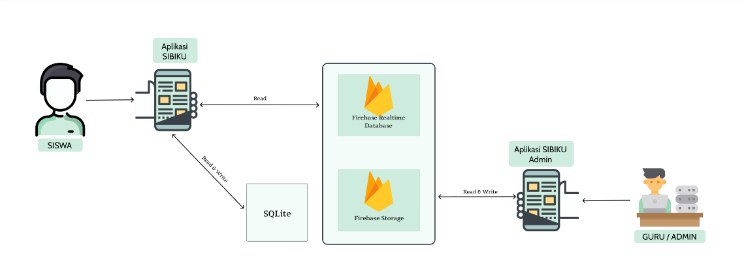
\includegraphics[width=8.58cm,height=2.68cm]{arsitektur}
    \caption{Arsitektur aplikasi.}
    \label{fig:arsitektur}
\end{figure}

Lorem ipsum dolor sit amet, consectetur adipiscing elit. Fusce sit amet magna
in diam finibus convallis. Nulla velit erat, efficitur vitae maximus ut,
imperdiet nec dolor. Sed dui ligula, rutrum eget quam eu, elementum finibus
ipsum. Integer sed porta risus, sit amet tristique neque. Nunc vel convallis
eros. Aliquam luctus lorem eu nisl porta dignissim sit amet ac tortor. Cras
auctor nibh ac aliquet interdum. Donec cursus mauris risus. Morbi laoreet augue
ac massa feugiat, ut laoreet magna semper. Ut non suscipit ante, et luctus
risus. Mauris porta tempus dictum.

\subsection{Struktur Data SQLite}
Vivamus tincidunt id nibh non euismod. Proin lectus orci, tempus ac rhoncus
vitae, luctus vel dolor. Phasellus faucibus porta urna, posuere consequat eros
dapibus at. Ut felis nisl, viverra vitae condimentum id, pretium et ex. Quisque
a maximus urna, quis rhoncus magna. In quis est sed augue aliquet aliquet in
quis diam. Praesent eget pulvinar mauris, eget sollicitudin nibh. Duis lacus
purus, sollicitudin sed erat eu, rutrum aliquet ex. Pellentesque habitant morbi
tristique senectus et netus et malesuada.

\begin{figure}[H]
    \centering
    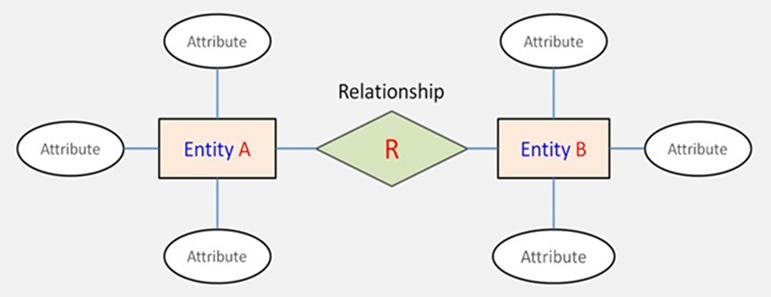
\includegraphics[width=8.58cm,height=3.31cm]{struktur-sqlite}
    \caption{Struktur Data SQLite.}
    \label{fig:struktur-sqlite}
\end{figure}

Donec sapien neque, dignissim efficitur nibh vitae, congue congue quam.
Pellentesque dolor urna, vulputate eget imperdiet at, congue sagittis nunc.
Suspendisse enim nulla, hendrerit eget erat quis, scelerisque varius diam.
Fusce tortor ex, aliquam non tristique at, elementum ut ex. Integer dignissim
dui sed iaculis tempor. Nullam vehicula, nibh quis tempor faucibus, est erat
commodo odio, nec volutpat nunc odio aliquet sem. Praesent metus enim, rutrum
eu ultrices at, rutrum nec ipsum. Vestibulum iaculis.

Vel mattis mauris mi in massa. Sed egestas non lacus ut dignissim. Donec
scelerisque auctor bibendum. Suspendisse in justo dolor. Praesent egestas justo
sed rhoncus maximus. Nunc lacinia convallis dui sed eleifend. Suspendisse rutrum
metus a facilisis viverra. Proin pellentesque accumsan orci eget suscipit.
Aliquam pulvinar nibh id est interdum sodales. Duis et sapien ac mauris imperdiet
tincidunt in eu neque. Integer porta lobortis nulla, vel dignissim neque
pellentesque vel. Donec erat magna, lobortis id tempus ut.

\subsection{Kebutuhan Pengembangan Aplikasi}
Untuk mengimplementasikan aplikasi sesuai rancangan yang telah dibuat, dibutuhkan
perangkat keras dan perangkat lunak berikut.

\begin{table}[H]
    \caption{Kebutuhan Hardware dan Software}
    \label{tab:kebutuhan}
    \centering
    \begin{tabular}{|p{0.45\linewidth}|p{0.45\linewidth}|}
        \hline
        \textbf{Hardware} & \textbf{Software} \\ \hline
        Laptop Asus ROG GL503GE:\newline Intel Core\textsuperscript{TM} i7 dan RAM 8GB
                          & Android Studio Arctic Fox - 2020.3.1 \\ \hline
        Smartphone Samsung A50:\newline layar 6.4'' dan RAM 4GB
                          & Firebase Realtime Database \\ \hline
        Oculus Quest 2     & Firebase Cloud Storage \\ \hline
        Arduino Uno        & Unity 2020.3 \\ \hline
                           & Arduino IDE \\ \hline
    \end{tabular}
\end{table}

% ===================== IMPLEMENTASI & PENGUJIAN =====================
\section{Implementasi dan Pengujian}
Bagian ini menjelaskan implementasi aplikasi, hingga pengujian yang dilakukan,
yaitu pengujian fungsionalitas dan pengujian ke pengguna.

\subsection{Implementasi Aplikasi}
Aplikasi SIBIKU terdiri dari dua bagian, yaitu aplikasi siswa dan aplikasi
guru/admin. Ini diimplementasikan di Android Studio dengan menggunakan pendekatan
single project multiple modules. Implementasi ini juga dilakukan dengan
arsitektur MVVM yang memisahkan kode terkait UI dengan kode terkait business
logic aplikasi. Kelas-kelas yang ada juga dibagi ke dalam package-package sesuai
fungsinya masing-masing.

\begin{figure}[H]
    \centering
    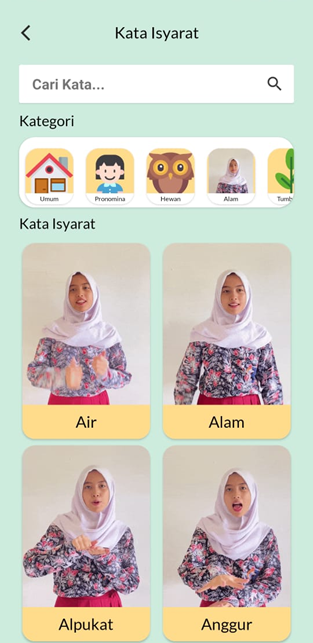
\includegraphics[width=4cm,height=8.22cm]{implementasi-1}\hspace{0.3cm}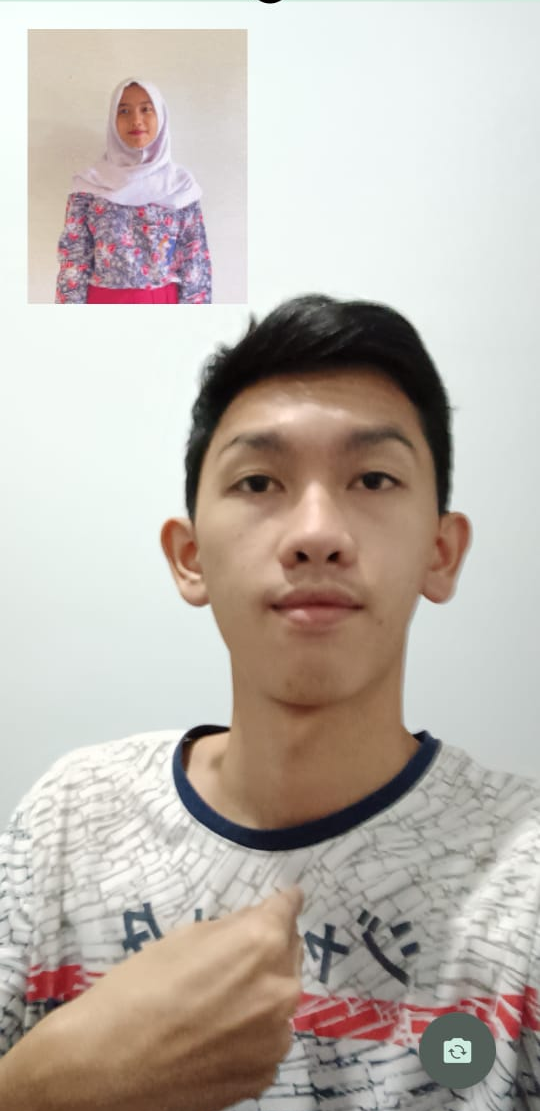
\includegraphics[width=4cm,height=8.23cm]{implementasi-2}
    \caption{Aplikasi hasil implementasi.}
    \label{fig:implementasi}
\end{figure}

Lorem ipsum dolor sit amet, consectetur adipiscing elit. Fusce sit amet magna
in diam finibus convallis. Nulla velit erat, efficitur vitae maximus ut,
imperdiet nec dolor. Sed dui ligula, rutrum eget quam eu, elementum finibus
ipsum. Integer sed porta risus, sit amet tristique neque. Nunc vel convallis
eros. Aliquam luctus lorem eu nisl porta dignissim sit amet ac tortor. Cras
auctor nibh ac aliquet interdum. Donec cursus mauris risus. Morbi laoreet augue.

Vivamus tincidunt id nibh non euismod. Proin lectus orci, tempus ac rhoncus
vitae, luctus vel dolor. Phasellus faucibus porta urna, posuere consequat eros
dapibus at. Ut felis nisl, viverra vitae condimentum id, pretium et ex. Quisque
a maximus urna, quis rhoncus magna. In quis est sed augue aliquet aliquet in
quis diam. Praesent eget pulvinar mauris, eget sollicitudin nibh duis lacus.

\subsection{Pengujian Aplikasi}
Pengujian aplikasi dilakukan dalam dua tahapan. Uji fungsionalitas aplikasi
dilakukan dengan metode black box. Pengujian diawali dengan membuat skenario
test untuk setiap fitur aplikasi, lalu menerjemahkan skenario tersebut ke dalam
instrumentation test menggunakan Espresso. Seluruh pengujian aplikasi ini
dilakukan menggunakan smartphone Redmi Note 10S dan sistem operasi Android 11.

Setelah uji fungsionalitas mendapatkan hasil yang valid, pengujian dilanjutkan
dengan pengujian ke pengguna. Ini dilakukan dengan metode usability test. Proses
pengujian diawali dengan membuat kuesioner di Google Form, lalu menyebarkan
kuesioner tersebut ke responden. Selanjutnya, dilakukan perhitungan hasil
kuesioner dengan skala Likert. Terakhir, dilakukan interpretasi hasil perhitungan.

Pengujian dilakukan dengan responden sebanyak 71 orang terdiri dari 35,2\% siswa
SLB, 12,7\% dosen/guru, 45,1\% mahasiswa, dan 7\% lainnya. Setiap responden
dipastikan telah mencoba aplikasi sebelum mengisi kuesioner, sebab pengujian
dilakukan secara sinkron melalui aplikasi Zoom. Berdasarkan hasil perhitungan,
sebanyak 89,7\% responden sangat setuju aplikasi telah berhasil menerapkan
effectiveness dalam fitur-fiturnya.

% ===================== KESIMPULAN =====================
\section{Kesimpulan}
Berdasarkan aplikasi yang telah dibangun dan pengujian yang telah dilakukan,
dapat disimpulkan bahwa aplikasi SIBIKU merupakan media belajar yang bagus dan
dapat membantu siswa SLB penyandang tunarungu dalam belajar bahasa isyarat
dengan mudah. Selain itu, aplikasi ini juga dapat membantu sekolah dan guru
dalam pembelajaran kosakata baru pada siswa SLB.

Aplikasi SIBIKU telah berhasil mencapai tujuannya. Ini dibuktikan pada pengujian
ke pengguna yang melibatkan 71 responden, dimana 91,30\% pengguna sangat setuju
bahwa aplikasi SIBIKU sangat efektif sebagai media dalam kegiatan belajar pada
siswa SLB penyandang tunarungu, berkat fitur tebak kata yang meningkatkan
semangat belajar dan juga sebagai evaluasi mandiri.

Untuk pengembangan aplikasi lebih lanjut, kosakata isyarat rencananya lebih
diperbanyak lagi, filter kata isyarat ditambah berdasarkan kelas, menambahkan
fitur ranking berdasarkan poin yang didapat dari keaktifan pengguna dalam
menggunakan aplikasi SIBIKU serta aplikasi dibuat dalam platform lain seperti
iOS.

% ===================== REFERENCES =====================
\begin{thebibliography}{7}
\bibitem{ref1}
G. Eason, B. Noble, and I. N. Sneddon, ``On certain integrals of
Lipschitz-Hankel type involving products of Bessel functions,'' Phil. Trans.
Roy. Soc. London, vol. A247, pp. 529--551, April 1955. (references)

\bibitem{ref2}
J. Clerk Maxwell, A Treatise on Electricity and Magnetism, 3rd ed., vol. 2.
Oxford: Clarendon, 1892, pp. 68--73.

\bibitem{ref3}
I. S. Jacobs and C. P. Bean, ``Fine particles, thin films and exchange
anisotropy,'' in Magnetism, vol. III, G. T. Rado and H. Suhl, Eds. New York:
Academic, 1963, pp. 271--350.

\bibitem{ref4}
K. Elissa, ``Title of paper if known,'' unpublished.

\bibitem{ref5}
R. Nicole, ``Title of paper with only first word capitalized,'' J. Name Stand.
Abbrev., in press.

\bibitem{ref6}
Y. Yorozu, M. Hirano, K. Oka, and Y. Tagawa, ``Electron spectroscopy studies on
magneto-optical media and plastic substrate interface,'' IEEE Transl. J. Magn.
Japan, vol. 2, pp. 740--741, August 1987 [Digests 9th Annual Conf. Magnetics
Japan, p. 301, 1982].

\bibitem{ref7}
M. Young, The Technical Writer's Handbook. Mill Valley, CA: University Science,
1989.
\end{thebibliography}

\end{document}
